\section{Giới thiệu và cơ sở lý thuyết tính toán song song}

\subsection{Đặt vấn đề}
Sự bùng nổ của các mô hình Trí tuệ Nhân tạo (AI), đặc biệt là các mô hình ngôn ngữ lớn và Generative AI, đã vượt quá khả năng xử lý của các hệ thống máy tính đơn lẻ. Kích thước tham số của các mô hình này tăng theo cấp số nhân, đòi hỏi một lượng lớn bộ nhớ (VRAM) và năng lực tính toán. Điều này dẫn đến sự cần thiết tất yếu của các hệ thống tính toán song song phân tán nhằm phân tải khối lượng công việc, tối ưu hóa thời gian huấn luyện và đáp ứng tốc độ phản hồi trong quá trình suy luận.

\subsection{Mục tiêu và phạm vi nghiên cứu}
Đồ án được thực hiện với hai mục tiêu chính:
\begin{itemize}
    \item Tổng hợp kiến thức nền tảng về tính toán song song và các framework phân tán tiên tiến hiện nay.
    \item Đề xuất và xây dựng một khung đánh giá hiệu năng (thí nghiệm) để kiểm chứng khả năng của các chiến lược song song hóa.
\end{itemize}
Phạm vi của báo cáo hiện tại tập trung ưu tiên nghiên cứu và tổng hợp cơ sở lý thuyết, phân tích cơ chế hoạt động của phần cứng và phần mềm. Phần thực nghiệm minh họa được cấu trúc dưới dạng khung dự kiến nhằm định hướng cho giai đoạn nghiên cứu và phát triển tiếp theo.

\subsection{Phương pháp nghiên cứu}
Phương pháp chủ đạo được áp dụng là nghiên cứu, thu thập và phân tích tài liệu kỹ thuật từ các nguồn uy tín như tài liệu của Phòng thí nghiệm Quốc gia Lawrence Livermore (LLNL), các ấn bản nghiên cứu trên arXiv, và mã nguồn mở từ NVIDIA, Microsoft, Meta. Dựa trên đó, đồ án thực hiện phân tích so sánh để làm rõ đặc tính của từng chiến lược song song hóa cũng như sự khác biệt giữa hai pha: huấn luyện (training) và suy luận (inference).

\subsection{Khái niệm cơ bản về lập trình song song}
Để hiểu rõ hệ thống phân tán, cần điểm qua các khái niệm cốt lõi:
\begin{itemize}
    \item \textbf{Kiến trúc máy tính:} Từ cấu trúc von Neumann truyền thống phân tách CPU và bộ nhớ, đến phân loại Flynn (như SIMD - Single Instruction, Multiple Data và MIMD - Multiple Instruction, Multiple Data) giải thích cách dữ liệu và luồng chỉ thị tương tác.
    \begin{figure}[H]
        \centering
        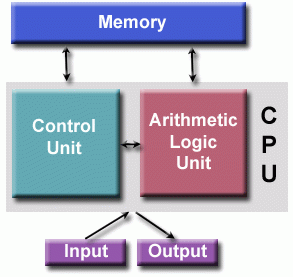
\includegraphics[width=0.6\textwidth]{Figures/vonNeumann1.png}
        \caption{Cấu trúc máy tính von Neumann truyền thống}
        \label{fig:von_neumann}
    \end{figure}
    \begin{figure}[H]
        \centering
        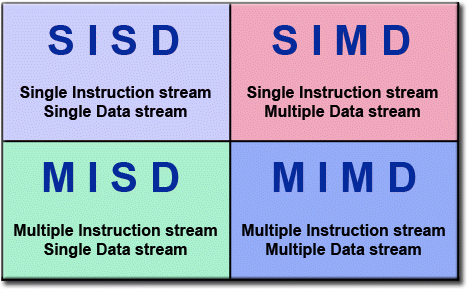
\includegraphics[width=0.7\textwidth]{Figures/flynnsTaxonomy.png}
        \caption{Phân loại kiến trúc máy tính theo Flynn}
        \label{fig:flynn}
    \end{figure}
    \item \textbf{Kiến trúc bộ nhớ:} Gồm hệ thống bộ nhớ chia sẻ (Shared Memory), hệ thống bộ nhớ phân tán (Distributed Memory) và các mô hình lai (Hybrid) thường thấy trên các siêu máy tính hiện đại.
    
    \begin{figure}[H]
        \centering
        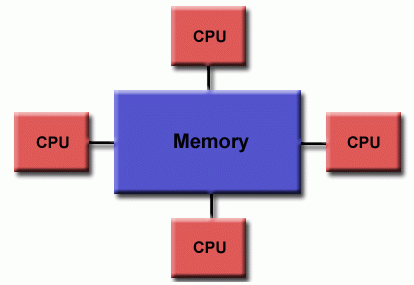
\includegraphics[width=0.5\textwidth]{Figures/shared_mem.png}
        \caption{Mô hình bộ nhớ chia sẻ (Shared Memory)}
        \label{fig:shared_mem}
    \end{figure}
    
    \begin{figure}[H]
        \centering
        
\includegraphics[width=0.6\textwidth]{"Figures/Non-Uniform Memory Access (NUMA).png"}
        \caption{Mô hình bộ nhớ chia sẻ không đồng nhất (NUMA - Hybrid)}
        \label{fig:numa_mem}
    \end{figure}

    \begin{figure}[H]
        \centering
        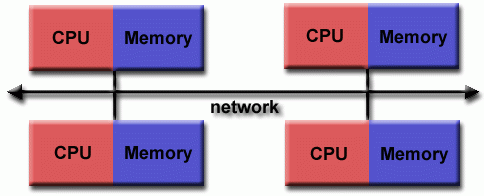
\includegraphics[width=0.5\textwidth]{Figures/distributed_mem.png}
        \caption{Mô hình bộ nhớ phân tán (Distributed Memory)}
        \label{fig:distributed_mem}
    \end{figure}
    \item \textbf{Mô hình lập trình:} Phổ biến nhất là OpenMP (hướng tới bộ nhớ chia sẻ) và MPI (hướng tới giao tiếp phân tán).
\end{itemize}

\subsection{Cấu trúc báo cáo}
Báo cáo được chia thành 4 phần chính. Phần 1 trình bày tổng quan và cơ sở lý thuyết. Phần 2 khảo sát các kỹ thuật lập trình song song trên CPU. Phần 3 đi sâu vào kiến trúc phần cứng GPU và các cơ chế giao tiếp liên GPU. Cuối cùng, Phần 4 phân tích các framework, các chiến lược phân tán cho AI, đưa ra so sánh giữa huấn luyện và suy luận, đồng thời đề xuất khung thực nghiệm minh họa.